\documentclass[a4paper]{article}
\usepackage[latin1]{inputenc}
\usepackage[T1]{fontenc}
\usepackage[francais]{babel}
\usepackage{entete}
\usepackage{noitemsep}
\usepackage{euscript} 
\usepackage{amsmath,amssymb,amsfonts,amsthm}
\usepackage{graphicx,graphics,epsfig,subfigure,color}
\usepackage{url}
%\usepackage{algorithm2e}
\usepackage{multicol}
\usepackage{a4wide}
\usepackage{latexsym}
\usepackage{verbatim}
\setlength{\textheight}{23.6cm}
\setlength{\topmargin}{-2cm}
\setlength{\textwidth}{160mm}
\setlength{\oddsidemargin}{1mm}
%\usepackage[clearempty]{titlesec}

\thispagestyle{empty}
%\renewcommand{\baselinestretch}{0.85}

%\input{macroAlgo}
%\dontprintsemicolon

\setlength{\parindent}{0pt}  %%suppression indentation


\begin{document}
\selectlanguage{francais}
\author{D. Fourer}
\newcommand{\universityname}{IUT d'\'Evry Val d'Essonne}
\newcommand{\deptname}{D\'epartement TC (S3)}
\newcommand{\years}{2022-2023}

%------------------- TITRE -----------------------------------------
\date{Septembre 2019} 
\TDHead{\universityname}{\deptname}{R3.12, RCN3, \years}{Nom: \hspace{5cm} Pr\'enom: \hspace{5cm} Groupe:\hspace{2cm}} %\large DS1: Utilisation avanc\'ee d'Excel
%\TDHead{DUT TC}{}{\large TIC3: Fonctions avanc\'ees d'un tableur}
%-------------------------------------------------------------------
\vspace{-0.6cm}
\begin{center}
 \textbf{TP not\'e, Dur\'ee: 1h30, documents interdits,\\objects connect\'es interdits.}
\end{center}
\vspace{-0.4cm}
\underline{Consignes:} 
\begin{itemize}
% \item Vous d\'eposerez les fichiers cr\'e\'es \textbf{dans un dossier portant votre nom} en veillant \`a indiquer le \textbf{num\'ero de poste}.
% \item Vous indiquerez pour chaque question le nom du fichier correspondant et une description succinte de ce qui a \'et\'e fait.
% \item Il n'est pas n\'ecessaire d'imprimer vos codes sources, qui devront \^etre propres et bien comment\'es, \textbf{1 point est r\'eserv\'e \`a la pr\'esentation et \`a l'indentation du code}.
 \item {\bf Le sujet devra imp\'erativement \^etre remis en fin de s\'eance. La non remise du sujet engendrera une note de 0/20}. % \textbf{Les copies remises sans le sujet ne seront pas corrig\'ees}.
 %\item Vous d\'eposerez votre fichier ``{\bf \verb?nom_prenom.xlsx?}'' sur E-Campus: \url{https://ecampus.paris-saclay.fr}.
 \item Vous enverrez votre travail ``{\bf \verb?nom_prenom.xlsx?}'' par e-mail \`a {\bf dominique.fourer@univ-evry.fr}.
% \item \textbf{1 point pour la pr\'esentation et le respect des consignes}.
\end{itemize}
\vspace{0.4cm}
%\vspace{1cm}

\exost (3 points)
%
\begin{enumerate}
 \item R\'ecup\'erez le fichier \verb?https://fourer.fr/dstic22.zip? et d\'ecompressez son contenu sur votre bureau. %%
 \item Ouvrez le fichier \verb?ds1.xlsx? dans lequel vous ajouterez une feuille de calcul \verb?ex1?.
 \item Importez le fichier \verb?resultats.csv? dans la nouvelle feuille \verb?ex1? en vous assurant que les donn\'ees soient utilisables (eg. dates, nombres, etc.).  %% 1
 \item Ajoutez une colonne ``\^age'' que vous calculerez pour chaque individu \`a partir de la date de naissance. %% 1
 \item Assurez-vous que les donn\'ees soient pr\'esent\'ees dans un tableau structur\'e disposant de filtres de tri.
\end{enumerate}

\exost (5 points)
%
\begin{enumerate}
 \item Cr\'eez une nouvelle feuille de calcul \verb?ex2?
 \item  Reproduisez \textbf{le tableau suivant}: \\ 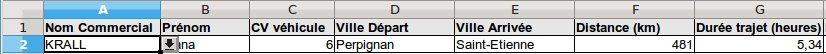
\includegraphics[width=0.95\textwidth]{feuille.png}
 \item \begin{enumerate}
        \item Limitez la cellule A2 pour qu'une liste d\'eroulante (tri par ordre alphab\'etique) vous permette de choisir un commercial par son \textbf{nom de famille}
        (depuis la feuille \verb?ex1?). 
        Les informations correspondantes (pr\'enom, CV, villes, etc.) devront se mettre \`a jour automatiquement.  %% 1pt
        \item Proposez une formule permettant d'obtenir la distance parcourue par le commercial entre la ville de d\'epart et la ville d'arriv\'ee,
        en effectuant une recherche dans le tableau de la feuille ``distance''.   %%[4 pts]
        %\item [0,5 pt]Calculez la dur\'ee estim\'ee du trajet en heures, pour une vitesse moyenne de 90 km/h\\
	\item En utilisant le gestionnaire de sc\'enarios, calculez 3 estimations de dur\'ee du trajet respectivement pour une vitesse moyenne de: 70km/h, 90km/h et 110km/h. 
	(Rappel: $t = \frac{d}{v}$, avec $t$ le temps en heures, $d$ la distance en km et $v$ la vitesse en km/h). %%1 pt
        %         \item \begin{minipage}{0.75\linewidth} %% 1pt
%         Vous calculerez l'indemnit\'e kilom\'etrique qui s'applique uniquement si la distance parcourue d\'epasse 50km ou si la dur\'ee du trajet d\'epasse 1h. Dans ce cas, appliquerez le montant kilom\'etrique qui correspond \`a la puissance fiscale du v\'ehicule:
%         \end{minipage} %% 3 pt
%         \begin{minipage}{0.25\linewidth}
%          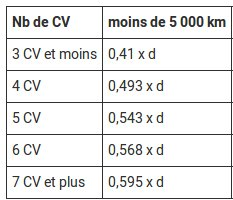
\includegraphics[width=\textwidth]{kilometres.jpg}
%         \end{minipage}     
%         % 
       \end{enumerate}
\end{enumerate}

\exost (3 points)
\begin{enumerate}
 \item Cr\'eez une nouvelle feuille de calcul \verb?ex3?.
 \item Produisez un tableau crois\'e dynamique qui affiche la moyenne des r\'esultats nets, en fonction de l'\^age des commerciaux. %% 1
 \item Repr\'esentez ces donn\'ees dans un diagramme en b\^atons (sur la m\^eme feuille avec l'\^age en abscisse).  %1
\end{enumerate}

%\exost (6 points) Cr\'eez une nouvelle feuille de calcul \verb?ex4? dans laquelle vous proposerez de trouver gr\^ace au solveur le commercial
%le plus proche de la ville choisie par l'utilisateur (menu d\'eroulant). Vous ajouterez librement sur cette feuille toutes les donn\'ees n\'ecessaires pour votre calcul.
%Vous effectuerez une recherche pour la ville de \textbf{Bordeaux} et vous enregistrerez la solution donn\'ee par le solveur.

\exost (4 points) Dans une nouvelle feuille de calcul \verb?ex4?, 
r\'esoudre le syst\`eme d'\'equations suivant avec excel en utilisant le nommage de cellules et le calcul it\'eratif: %1pt
\begin{align}
 \cos(2\pi x)  + 3y	&= 330\\
 \frac{3}{2} x - 7y  	&= 680
\end{align}

\exost (5 points) Cr\'eez une nouvelle feuille de calcul \verb?ex5? dans laquelle vous proposerez un formulaire
permettant \`a partir de la ville s\'electionn\'ee dans un menu d\'eroulant, de trouver le NOM du commercial le plus proche. Vous ajouterez
librement sur cette feuille toutes les donn\'ees n\'ecessaires pour effectuer ce calcul.

% \section{Mise en place de l'environnement de travail} %%duree 30min, 1h maxi
% 
% %% chargement d'un fichier audio et creation d'un script.
% \exost Cr\'eez un r\'epertoire sur le bureau portant le nom \verb? TD_excel_NOM_PRENOM ? Vous y d\'eposerez le contenu
% de l'archive contenant les fichiers du TD disponible sur \url{http://www.fourer.fr/Ens/1819/TIC/td_excel.zip} que vous prendrez 
% soin de d\'ecompresser.
% Assurez vous que vous parvenez \`a ouvrir le fichier avec le logiciel tableur (Microsoft Excel ou Libreoffice Calc).
% 
% \exost Ouvrez le fichier \verb? classe.xls ? Effectuez un tri des noms des \'etudiant par ordre alphab\'etique (ordre lexicographique croissant)
% en conservant sur chaque ligne l'affectation initiale des notes pour chaque \'etudiant.
% 
% 
% \section{Formules math\'ematiques} %%duree 30min, 1h maxi
% 
% \exost Ins\'erez une nouvelle colonne avant la colonne \verb? NOM ? que vous appelerez \verb? ID ?.
% Affectez un num\'ero disctinct \`a chaque \'etudiant. Vous commencerez par affecter un nombre au premier \'etudiant
% puis vous appliquerez la formule $=x+1$ \`a l'\'etudiant suivant ($x$ repr\'esente le code de la cellule associ\'e \`a l'ID pr\'ec\'edent).
% En utilisant la fonction copier-coller, vous appliquerez cette formule \`a l'ensemble des \'etudiants.
% 
% \exost Ins\'erez une nouvelle colonne apr\`es la derni\`ere note que vous appelerez \verb? MOYENNE ?. 
% Vous ins\`ererez la moyenne pour toutes les mati\`eres dans cette colonne en utilisant une formule de la forme
% \verb? =MOYENNE(x:y) ? o\`u $x$ et $y$ sont respectivement les codes de la premi\`ere et de la derni\`ere cellule prises en compte pour le calcul
% de la moyenne.
% 
% %%duree 30min, 1h maxi
% \exost Ajoutez une nouvelle colonne \verb? MEDIANE ?
% 
% \exost Ajoutez une nouvelle colonne \verb? MOYENNE PONDEREE ? Pour cela vous impl\'ementerez la formule suivante:
% 
% \begin{equation}
%  \bar{x} = \frac{\sum_i c_i x_i}{\sum_i c_i} = \frac{c_1 x_1 + c_2 x_2 + ...}{c_1 + c_2 + ...}
% \end{equation}
% 
% o\`u les $c_i$ correspondent au coefficient de chaque mati\`ere que vous r\'ecup\`ererez dans la seconde feuille de calcul et
% les $x_i$ correspondent aux notes correspondant \`a chaque mati\`ere $i$.
% 
% 
% \section{}




\end{document}

% End Of File

